\documentclass[]{article}
\usepackage[a4paper]{geometry}
\usepackage[dutch]{babel}
\usepackage{listings}

% Pretty figures
\usepackage{graphicx}
\usepackage{caption}
\usepackage{subcaption}

% Links
\usepackage{hyperref}

\setlength{\parindent}{0pt}
\setlength{\parskip}{14pt}

\title{
    Programmadocumentatie
}

\author{}
\date{}

\begin{document}

\maketitle

\tableofcontents
\clearpage

\section{Niet-ingelogde gebruiker}

\subsection{Registreren}

\begin{figure}[!ht]
	\centering
	
\includegraphics[width=0.5\textwidth]{img/registreerknop}
	\caption{Knop om te registreren}
	\label{registreerknop}
\end{figure}

\begin{figure}[!ht]
	\centering
	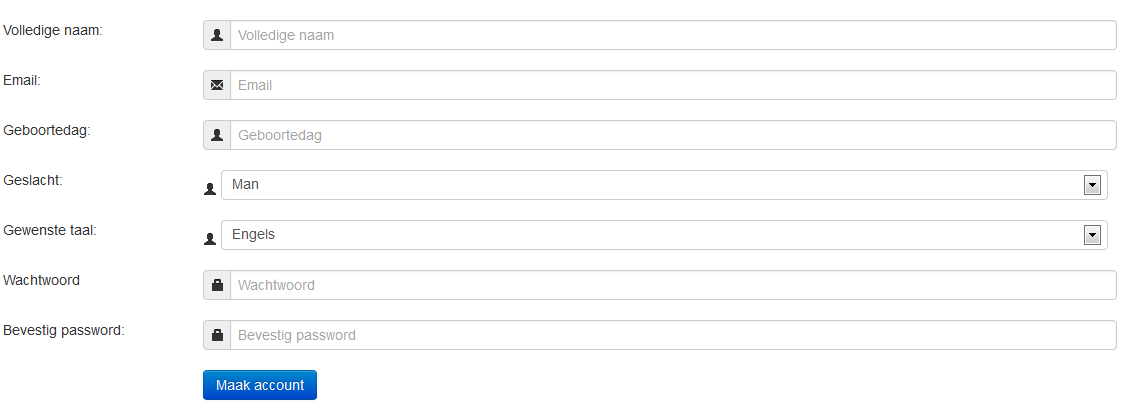
\includegraphics[width=1\textwidth]{img/registerform}
	\caption{Registratieformulier}
	\label{registerform}
\end{figure}

Om te registreren en een Bebras account aan te maken klik je op 'Registreer'. Hierdoor kom je op de pagina om een account aan te maken. Hier vul je de gevraagde velden in te beginnen met je naam. Vervolgens vul je jouw e-mailadres in, indien je hierover beschikt. Zo niet, dan mag je dit veld leeg laten. Om je geboortedatum in te geven, kan je gebruik maken van de datumkiezer of je kan deze zelf ingeven volgens het 'DD/MM/YYYY'-formaat. Je duidt je geslacht aan (Man/Vrouw/Ander) en kiest de taal die je voorkeur wegdraagt. Hiervoor kan je kiezen uit Nederlands, Frans of Duits. Onderaan vul je een zelfgekozen wachtwoord in. Dit herhaal je in het veld eronder. Klik dan op 'Maak account'. Je krijgt een Bebras-ID toebedeeld en kan hiermee inloggen.

\textbf{\textit{Wat kan er mislopen?}}

\begin{itemize}
\item Verplichte velden die niet ingevuld zijn: Vul alle verplichte velden in.
\item Ongeldig e-mailadres: Vul een geldig e-mailadres in.
\item Het opgegeven e-mailadres is reeds in gebruik: Vul een ander e-mailadres in.
\item Ongeldige datum: Vul de datum in volgens het 'DD/MM/YYYY'-formaat.
\item Wachtwoorden komen niet overeen: Wees zeker dat je tweemaal hetzelfde wachtwoord invult.
\end{itemize}

\subsection{Inloggen}

\begin{figure}[!ht]
	\centering
	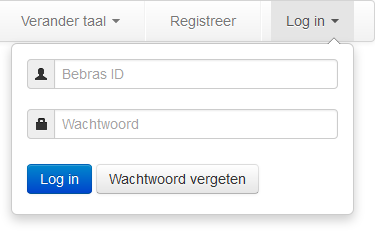
\includegraphics[width=0.5\textwidth]{img/loginscreen}
	\caption{Inloggen}
	\label{loginscreen}
\end{figure}

Nu je een Bebras account hebt aangemaakt, kun je ook inloggen. Hiervoor klik je op de startpagina op 'Log in'. Vul je Bebras-ID en wachtwoord in, klik op 'Log in' en je bent ingelogd! Als alles goed gaat, zie je nu jouw persoonlijke pagina. 

\textbf{\textit{Wat kan er mislopen?}}

Als er een veld niet ingevuld is, zal je hier een melding van krijgen. Zorg ervoor dat alle verplichte velden ingevuld zijn.

In het geval dat je een foute gebruikersnaam of wachtwoord hebt ingevuld, zal je hiervan een melding krijgen. Probeer opnieuw in te loggen met de correcte gegevens of klik op 'Wachtwoord vergeten' indien je jouw wachtwoord niet meer weet.

Het kan ook gebeuren dat jouw account momenteel bezet is en nagebootst wordt door iemand die hoger in de hi"erarchie staat. Wanneer deze situatie zich voordoet, zal je momenteel niet kunnen inloggen. Probeer op een ander moment opnieuw.

\subsection{Wachtwoord vergeten}

\begin{figure}[!ht]
	\centering
	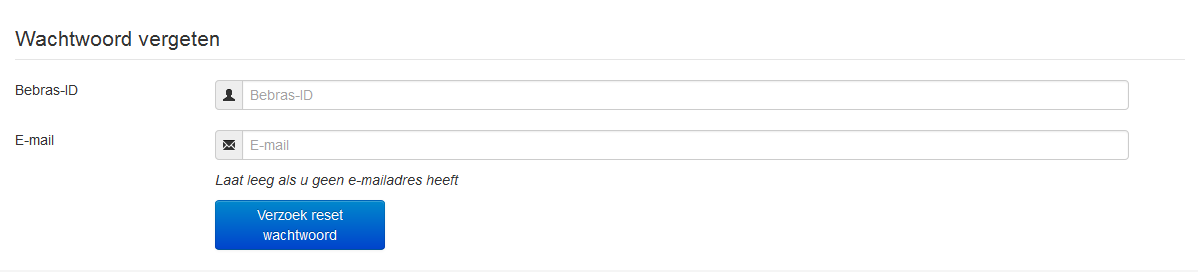
\includegraphics[width=1\textwidth]{img/forgotpwd}
	\caption{Wachtwoord vergeten}
	\label{forgotpwd}
\end{figure}

In het geval dat je je wachtwoord niet meer weet, kan je klikken op 'Wachtwoord vergeten' dat zich op het aanmeldvenster bevindt naast de loginknop. Hier vul je jouw Bebras-ID in en je e-mailadres. Indien je geen e-mailadres hebt opgegeven bij de registratie, omdat je zelf niet over een e-mailadres beschikt, laat je dit veld leeg. Je leerkracht zal dan instructies toegestuurd krijgen om je wachtwoord te resetten.

Je zal nu een e-mail in je inbox vinden met een eenmalige link waar je je wachtwoord opnieuw kan instellen. Kies een nieuw wachtwoord, vul dit nogmaals in om te bevestigen en klik op 'Ok'. Je kan nu inloggen met je nieuwe wachtwoord.

\textbf{\textit{Wat kan er mislopen?}}

Als er een veld niet (correct) ingevuld is, zal je hier een melding van krijgen. Zorg ervoor dat alle verplichte velden (correct) ingevuld zijn.

Heb je geen mail ontvangen? Kijk dan zeker eens in de map voor ongewenste e-mail. Het zou kunnen voorvallen dat de e-mail hier verzeild is geraakt. Als hier ook niets te vinden is, heb je misschien een foutief e-mailadres opgegeven. Je kan een nieuwe mail laten versturen door de procedure opnieuw te doorlopen.

\subsection{Verander taal}

\begin{figure}[!ht]
	\centering
	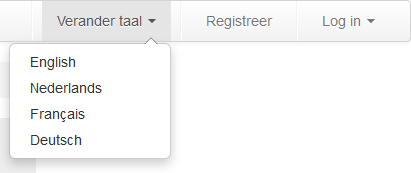
\includegraphics[width=0.5\textwidth]{img/change_lang}
	\caption{Taal veranderen}
	\label{change_lang}
\end{figure}

Hier kan je de taal van de website aanpassen. Je hebt de keuze uit Nederlands, Frans en Duits.

\subsection{Links}

\begin{figure}[!ht]
	\centering
	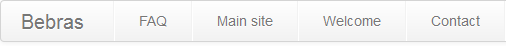
\includegraphics[width=0.75\textwidth]{img/links}
	\caption{Enkele links}
	\label{links}
\end{figure}

\begin{figure}[!ht]
	\centering
	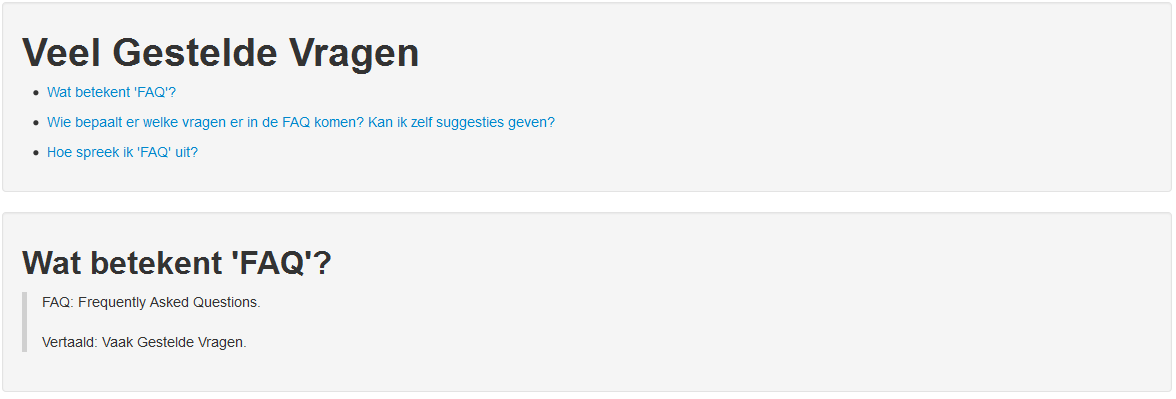
\includegraphics[width=1\textwidth]{img/faq}
	\caption{Veelgestelde vragen bekijken}
	\label{faq}
\end{figure}

Linksbovenaan staan een aantal links. Zo kun je op elk moment terugkeren naar de startpagina of de FAQ bekijken. Ook is er een link naar de offici"ele website waar men meer info kan vinden over de organisatie.

\subsection{Contact}

\begin{figure}[!ht]
	\centering
	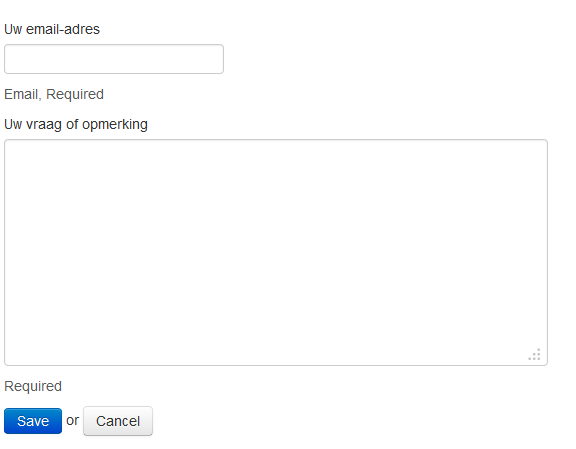
\includegraphics[width=1\textwidth]{img/contact}
	\caption{Contactformulier}
	\label{contact}
\end{figure}

Hier kan je contact opnemen met de organisatie. Formuleer je klacht, vraag, aan- of opmerking en vul zeker je e-mailadres in zodat we een antwoord kunnen terugsturen. 

\textbf{\textit{Wat kan er mislopen?}}

\begin{itemize}
\item Verplichte velden die niet ingevuld zijn: Vul alle verplichte velden in.
\item Ongeldig e-mailadres: Vul een geldig e-mailadres in.
\end{itemize}

\section{Leerling}

Nu je aangemeld bent, beschik je over een aantal standaardfuncties.

\subsection{Instellingen}

Deze kan je bereiken door op je dashboard op 'Instellingen' te klikken of door rechtsboven op je Bebras-ID te klikken zodat er een menu wordt geopend en daar voor 'Instellingen' te kiezen.

\subsubsection{Profiel bewerken}

\begin{figure}[!ht]
	\centering
	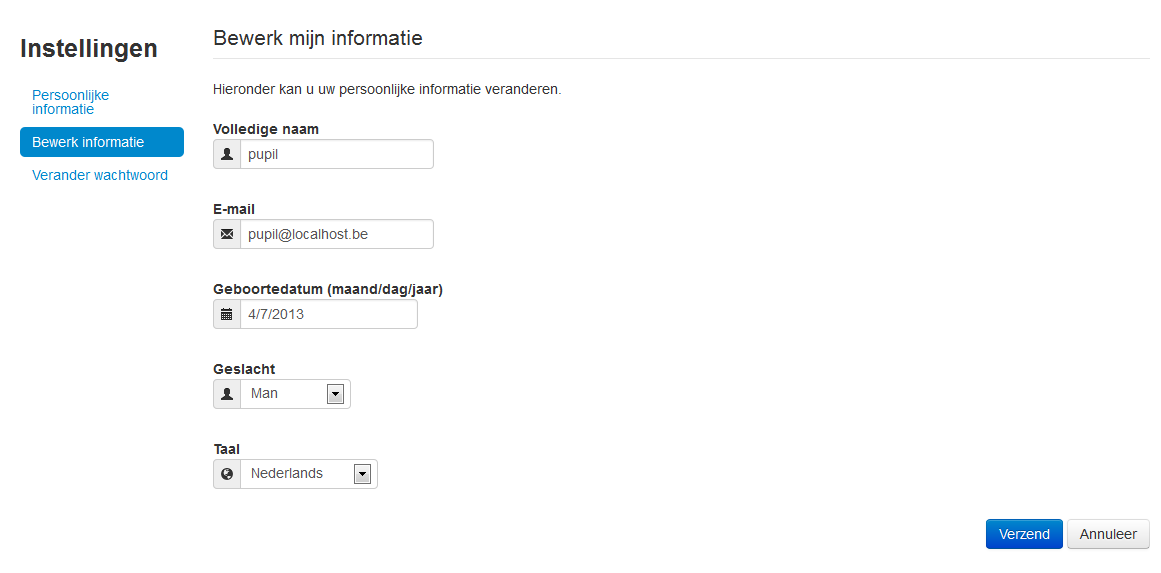
\includegraphics[width=1\textwidth]{img/pie}
	\caption{Profiel bewerken}
	\label{pie}
\end{figure} 
			
Hier kan je de verschillende gegevens die op jouw profiel verschijnen, zoals opgegeven bij registratie, aanpassen. Om de aanpassingen op te slaan, klik je op 'Verzend'.

\textbf{\textit{Wat kan er mislopen?}}

\begin{itemize}
\item Verplichte velden die niet ingevuld zijn: Vul alle verplichte velden in.
\item Ongeldig e-mailadres: Vul een geldig e-mailadres in.
\item Het opgegeven e-mailadres is reeds in gebruik: Vul een ander e-mailadres in.
\item Ongeldige datum: Vul de datum in volgens het 'DD/MM/YYYY'-formaat.
\end{itemize}

\subsubsection{Wachtwoord veranderen}

\begin{figure}[!ht]
	\centering
	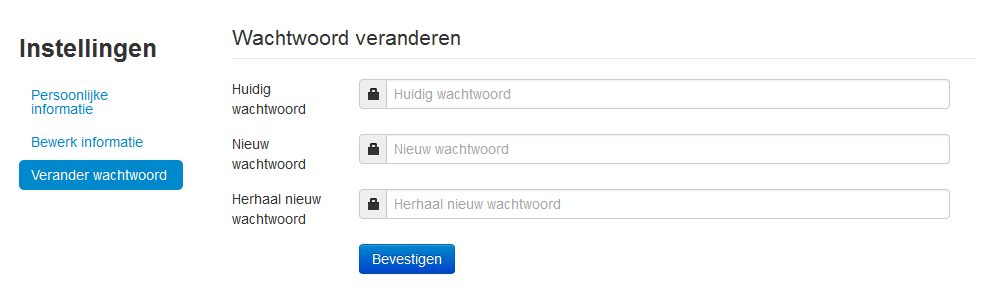
\includegraphics[width=1\textwidth]{img/changepwd}
	\caption{Wachtwoord veranderen}
	\label{changepwd}
\end{figure} 

Om je wachtwoord te veranderen, vul je jouw huidig wachtwoord in. Geef dan je nieuwe wachtwoord in en bevestig dit in het veld eronder. Klik op 'Ok' om je wachtwoord te wijzigen.

\textbf{\textit{Wat kan er mislopen?}}

\begin{itemize}
\item Verplichte velden die niet ingevuld zijn: Vul alle verplichte velden in.
\item Huidig wachtwoord is onjuist: Vul je huidige wachtwoord correct in.
\item Nieuw wachtwoord wordt niet correct bevestigd: Vul tweemaal je nieuwe wachtwoord correct in.
\end{itemize}

\subsection{Uitloggen}

\begin{figure}[!ht]
	\centering
	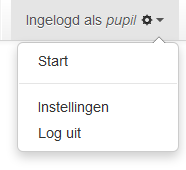
\includegraphics[width=0.25\textwidth]{img/logout}
	\caption{Uitloggen}
	\label{logout}
\end{figure} 

Om de webapplicatie te verlaten, klik je rechtsbovenaan op je gebruikersnaam. Er zal een menu verschijnen waar je onderaan voor 'Log uit' kunt kiezen.

\section{Auteur}

Dit type van account is speciaal voorbehouden voor gebruikers die enkel het maken van vragen als hoofddoel hebben.

\subsection{Vrageneditor}

\begin{figure}[!ht]
	\centering
	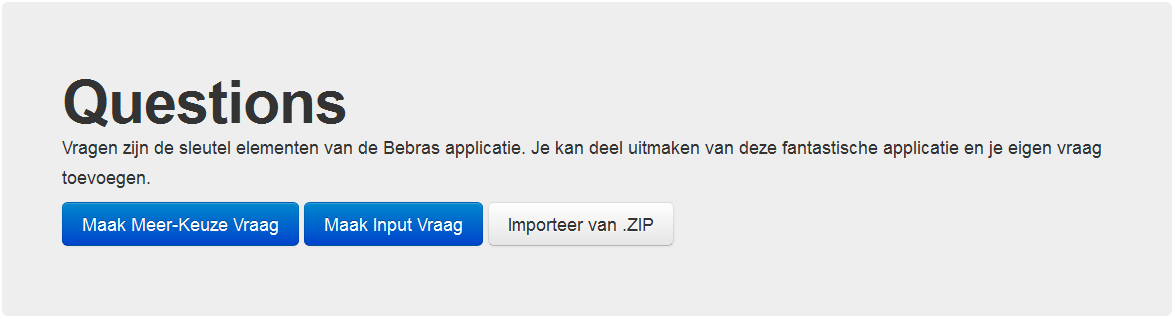
\includegraphics[width=1\textwidth]{img/questioneditor}
	\caption{Vrageneditor}
	\label{questioneditor}
\end{figure}

Om een eigen vraag toe te voegen ga je naar de 'Vrageneditor'. Bij het maken van een vraag, heb je verschillende keuzes. Of je maakt een meerkeuzevraag, of een open vraag. Voor meer ervaren gebruikers is er ook de mogelijkheid een vraag te uploaden in de vorm van een ZIP-bestand.

\subsubsection{Meerkeuzevraag}

\begin{figure}[!ht]
	\centering
	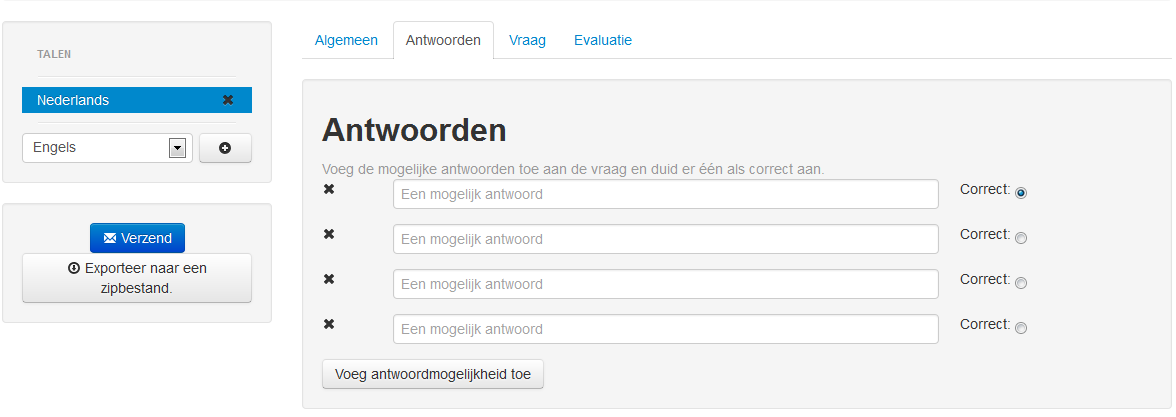
\includegraphics[width=1\textwidth]{img/mcq}
	\caption{Meerkeuzevraag opstellen}
	\label{mcq}
\end{figure}

Om een meerkeuzevraag aan te maken, kies je eerst de taal waarin de vraag wordt opgesteld. Klik dan op de plus knop om een vraag in deze taal toe te voegen. Nu zie je 4 tabbladen verschijnen, namelijk: 'Algemeen', 'Antwoorden', 'Vraag' en 'Evaluatie'. Bij het tabblad 'Algemeen' vul je de titel van de vraag in. Onder 'Antwoorden' is het de bedoeling dat je de 4 mogelijke antwoorden geeft en aanvinkt welke van de 4 de correcte oplossing is. Bij het tabblad 'Vraag' kun je de vraag ingeven in het hiervoor voorziene tekstvak. Boven het tekstvak vind je enkele knoppen om de opmaak te verzorgen. Het tabblad 'Evaluatie' lijkt sterk op het vorige. Hier is het de bedoeling dat je de feedback ingeeft die de participant te zien krijgt nadat hij deze vraag beantwoord heeft in een wedstrijd. 

Eens alles ingevuld is, klik je op 'Verzend'. Indien er zich geen foutmeldingen voordoen, is de vraag succesvol ingediend. In het andere geval zal je gevraagd worden om alles nog eens na te lezen en de hiaten in te vullen.

Als je dezelfde vraag in een andere taal wil toevoegen, kies je die taal en voeg je deze toe door dezelfde procedure te volgen. Wil je de vraag in een bepaalde taal verwijderen, klik dan op het kruisje dat naast de taal staat en bevestig je actie. 

Voorts heeft men ook nog de mogelijkheid om de opgestelde vraag in de verschillende talen te downloaden in de vorm van een ZIP-bestand. 

\subsubsection{Open vraag}

Bij het maken van een open vraag, kan men dezelfde procedure volgen als bij het maken van een meerkeuzevraag. Het enige verschil is dat men onder 'Antwoord' geen 4 keuzemogelijkheden ingeeft, maar 1 correct antwoord.

\subsubsection{Importeren}
Om een vraag te uploaden, klik je op 'Importeer van .ZIP'. Er zal een dialoogvenster verschijnen waar men het gewenste bestand kan zoeken en uploaden. Dit ZIP-bestand moet aan bepaalde eisen voldoen. Zo zal er per taal een indexpagina en een pagina voor feedback aanwezig moeten zijn. Vanuit deze HTML-bestanden kan verwezen worden naar andere bestanden, zoals afbeeldingen, die in het ZIP-bestand kunnen meegeleverd worden. Subfolders zijn hierbij niet toegelaten. Daarenboven moet er zich ook een XML-gebaseerd configuratiebestand in het ZIP-bestand bevinden. 

Dit XML-bestand, dat altijd de naam "`question.xml"' moet hebben, bevat
\begin{itemize}
\item de beschikbare talen
\item de startpagina van de vraag per taal
\item de titel van de vraag voor alle beschikbare talen
\end{itemize}

Voorts wordt er onderscheid gemaakt tussen meerkeuzevragen en open vragen.

\textbf{Structuur:}

Het XML-bestand bestaat uit een wortelknoop \verb+<root xmlns="bebras:Question">+ 
die op zijn beurt de soort vraag herbergt: \verb+<multiple-choice-question>+ of \verb+<regex-question>+.
Het 'vraag'-element bevat per beschikbare taal (\verb+<language code="xx">+) 
de start- en feedbackpagina (\verb+<index>index_xx.html</index>+ en \verb+<feedback>feedback_xx.html</feedback>+), 
de titel van de vraag tussen \verb+<title>+ tags 
en het antwoord (\verb+<input regex=""/>+) / de mogelijke antwoorden (\verb+<answers><answer></answer></answers>+)
met een indicatie bij het correcte antwoord door de optie \verb+correct="true"+ mee te geven.

Voorbeelden:
\lstinputlisting[language=XML, frame=single]{xml/MCQ.xml}
\lstinputlisting[language=XML, frame=single]{xml/open_question.xml} 

\begin{itemize}
\item Verplichte velden die niet ingevuld zijn: Vul alle verplichte velden in.
\item De vraag moet in minstens 1 taal compleet opgesteld zijn om te kunnen verzenden of exporteren.
\item Bij elke meerkeuzevraag moet in iedere beschikbare taal een correct antwoord aangeduid worden.
\item Importeren mislukt: Zorg ervoor dat het ZIP-bestand aan de vooropgestelde eisen voldoet.
\end{itemize}

\section{Leerkracht}

Als leerkracht beschik je over volgende extra functies.

\subsection{Lijst van scholen}

\begin{figure}[!ht]
	\centering
	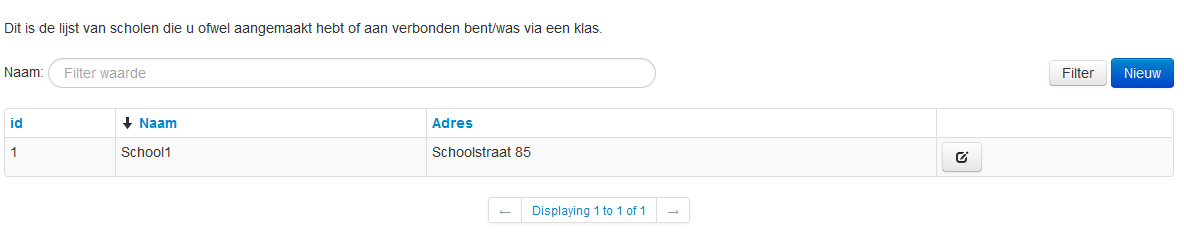
\includegraphics[width=1\textwidth]{img/schools}
	\caption{Lijst van scholen}
	\label{schools}
\end{figure}

Hier vindt de leerkracht de lijst van scholen waaraan hij/zij les heeft gegeven.

Om een nieuwe school aan het systeem toe te voegen, klik je op 'Nieuw'. Vul de naam en het adres van de school in en klik op 'Save'. De nieuwe school zal dan verschijnen in het overzicht als er een verbintenis met de school is.

\textbf{\textit{Wat kan er mislopen?}}

Zorg ervoor dat alle verplichte velden ingevuld zijn. Het is niet de bedoeling dat scholen tweemaal in het systeem opgenomen worden. Als de school al aanwezig is in het systeem, vraag dan naar het ID.

\subsection{Lijst van klassen}

[TODO: screenshot klasoverzicht]
Op deze pagina kan een leerkracht een overzicht krijgen van alle klassen met vermelding van de school, verantwoordelijke leraar en de leeftijdscategorie. Daarnaast staat ook de geldigheidsdatum vermeld en of de klas momenteel actief is.
Men kan in de lijst zoeken naar klassen van een bepaalde leerkracht door te filteren op zijn/haar Bebras-ID.

[TODO: screenshot nieuwe klas]
Om een nieuwe klas aan te maken, klik je rechtsboven op 'Nieuw'. Daar geef je de naam van de nieuwe klas, de school, leeftijdscategorie en geldigheidsdatum in en klik je op 'Save'.

Men kan ook een klas toevoegen door een Excel-bestand te uploaden. Dit bestand moet voldoen aan het vaste formaat dat hier beschreven wordt. 
Vooreerst is het belangrijk om te weten dat enkel en alleen het eerste werkblad zal verwerkt worden. Alle nodige gegevens zullen dus hier terecht moeten komen. De gegevens worden per rij verwerkt. Elke rij komt dus overeen met een record. Er wordt onderscheid gemaakt tussen 3 soorten records: 'Pupil'-records, 'Class'-records en records voor commentaar.

Een 'Pupil'-record bevat in de eerste cel het woord 'Pupil'. De volgende kolommen hebben achtereenvolgens als inhoud: ID, naam, geboortedatum, geslacht, voorkeurstaal, wachtwoord en e-mailadres. Om een bestaande gebruiker als leerling toe te voegen aan de klas, volstaat het om zijn Bebras-ID in te vullen. De rest van het record zal dan genegeerd worden. Als het ID gevonden wordt bij een leerling in het systeem, wordt die toegevoegd aan de nieuwe klas en, indien hij nog actief zou zijn in een andere klas, als oud-leerling ingesteld bij zijn huidige klas.  
Om een nieuwe gebruiker toe te voegen, laat je het veld ID leeg. De overige kolommen zijn verplicht, met uitzondering van e-mailadres.

Een 'Class'-record bevat in de eerste cel het woord 'Class'. De volgende kolommen hebben achtereenvolgens als inhoud: naam, geldigheidsdatum, leeftijdscategorie en het ID van de school. Alle kolommen moeten correct ingevuld worden en de klas zal enkel toegevoegd worden als de leeftijdscategorie en het ID van de school in het systeem aanwezig zijn. 

De overige records worden beschouwd als commentaar en zullen genegeerd worden.

Alle 'Pupil'-records die onder een 'Class'-record staan, worden beschouwd als leerlingen van deze klas. 

[TODO: screenshot klasinfo]
Een klas aanpassen kan door in de lijst op de 'Bewerk'-knop te klikken bij de betreffende klas. Hier vindt men meer info over de klas, school en leraar. Daarenboven is hier ook de lijst van studenten uit deze klas te vinden, alsook de hulpleerkrachten en de oud-studenten. Deze kunnen toegevoegd worden aan de hand van hun Bebras-ID.

Door hier een Excel-bestand te uploaden zoals reeds beschreven, kan men leerlingen toevoegen aan de bestaande klas. 'Class'-records zullen hierbij genegeerd worden.

De mogelijkheid bestaat ook om een Excel-bestand met alle informatie van de klas te downloaden.

\textbf{\textit{Wat kan er mislopen?}}

Alle verplichte velden moeten zeker en vast ingevuld zijn.

Het ID van de school en de leerkracht moet bestaan in het systeem. Verzeker je er dus van dat je zeker de juiste ID's ingeeft als je een foutmelding hieromtrent krijgt.

Na het uploaden van het Excel-bestand, wordt er een bevestigingspagina getoond. Dit is een overzicht met alle records die zullen toegevoegd worden en welke niet wegens fouten. Als een 'Class'-record foutief is, worden de bijhorende leerlingen niet opgeslaan. Men kan eventueel een nieuw bestand uploaden of doorgaan met opslaan.

Als het bestand niet kon ingelezen worden, zal je hiervan een melding krijgen. Controleer of de records voldoen aan de richtlijnen en sla het bestand op in xlsx-formaat.

Het kan ook occassioneel gebeuren dat de gegevens niet kunnen opgeslaan worden. Dit is waarschijnlijk te wijten aan een interne fout. Probeer opnieuw of contacteer de administrator bij aanhoudende problemen. 

\section{Organisator}

Als organisator beschik je over volgende extra functies.

\subsection{Gebruikersbeheer}
Op deze pagina krijgt de organisator een volledig overzicht van alle geregistreerde gebruikers. Hij kan een nieuwe gebruiker van elk type aanmaken door op 'Nieuw' te klikken en een gereduceerd registratieformulier in te vullen. Ook heeft de organisator de mogelijkheid om de gegevens en het wachtwoord van gebruikers aan te passen of zelfs accounts (tijdelijk) te blokkeren. 

\begin{figure}[!ht]
	\centering
	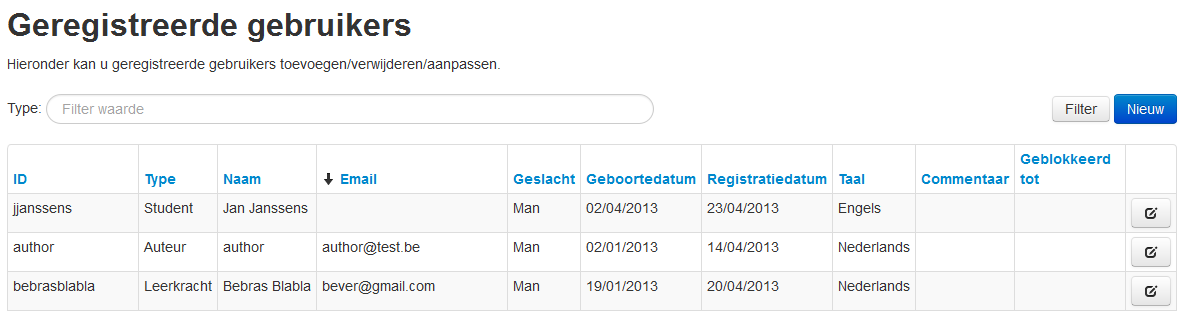
\includegraphics[width=1\textwidth]{img/usermgmt}
	\caption{Overzicht van gebruikers}
	\label{usermgmt}
\end{figure}

\begin{figure}[!ht]
	\centering
	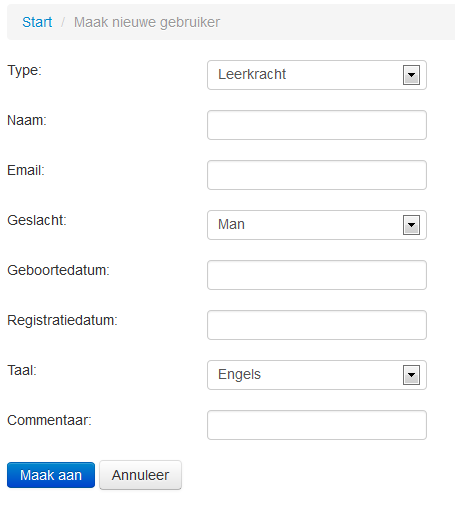
\includegraphics[width=0.5\textwidth]{img/create_user}
	\caption{Nieuwe gebruiker aanmaken}
	\label{create_user}
\end{figure}

\begin{figure}[!ht]
	\centering
	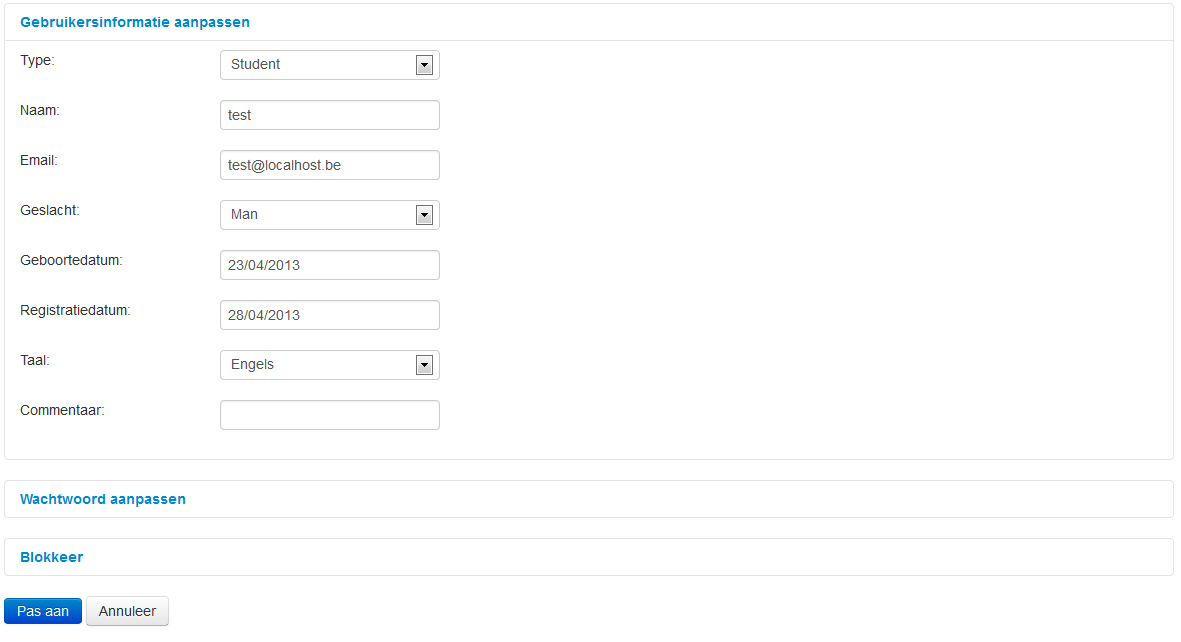
\includegraphics[width=1\textwidth]{img/edit_user}
	\caption{Gebruiker aanpassen}
	\label{edit_user}
\end{figure}

\begin{figure}[!ht]
	\centering
	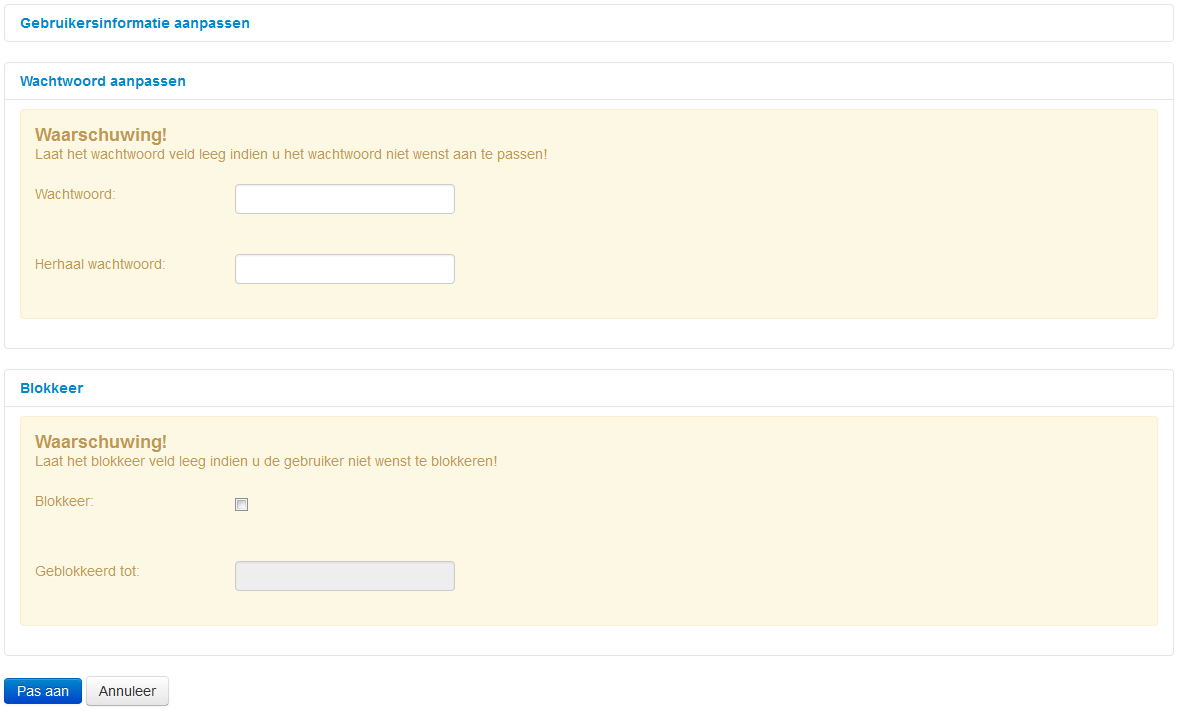
\includegraphics[width=1\textwidth]{img/block_user}
	\caption{Gebruiker blokkeren}
	\label{block_user}
\end{figure}

\subsection{Serverbeheer}

\subsubsection{Bekijk servers}
Deze pagina geeft een overzicht van de servers die momenteel gebruikt worden. Bovenaan kan men filteren op naam alsook een nieuwe server toevoegen. [TODO: screenshot server]

\subsubsection{Voeg server toe}

\begin{figure}[!ht]
	\centering
	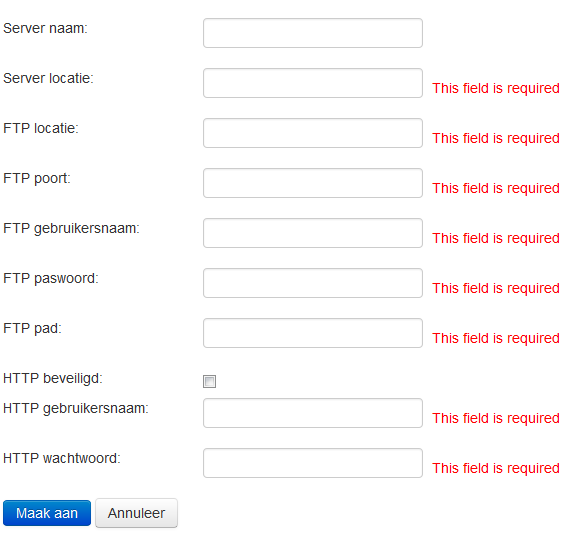
\includegraphics[width=0.5\textwidth]{img/new_server}
	\caption{Nieuwe server toevoegen}
	\label{new_server}
\end{figure}

Om een nieuwe server toe te voegen, vul je de gevraagde velden in. Kies vooreerst een naam voor de server. Vervolgens moet je de locatie van de server opgeven. Tot slot worden er nog enkele FTP-gegevens gevraagd: locatie, poortnummer, gebruikersnaam, paswoord en pas. Klik op 'Maak aan' om de server toe te voegen. Om de actie te annuleren, klik je op 'Annuleer'.

\textbf{\textit{Wat kan er mislopen?}}

Zorg er zeker voor dat alle verplichte velden zijn ingevuld. Bij de melding dat de base url of het pad ongeldig is, kijk je dit best nog eens na en verbeter waar nodig.

\subsection{Vragenbeheer}

\subsubsection{Bekijk vragen}
Deze pagina geeft een overzicht van de servers die momenteel gebruikt worden. Bovenaan kan men filteren op ID. [TODO: screenshot questions]

\subsubsection{Goedkeuren van vragen}

\begin{figure}[!ht]
	\centering
	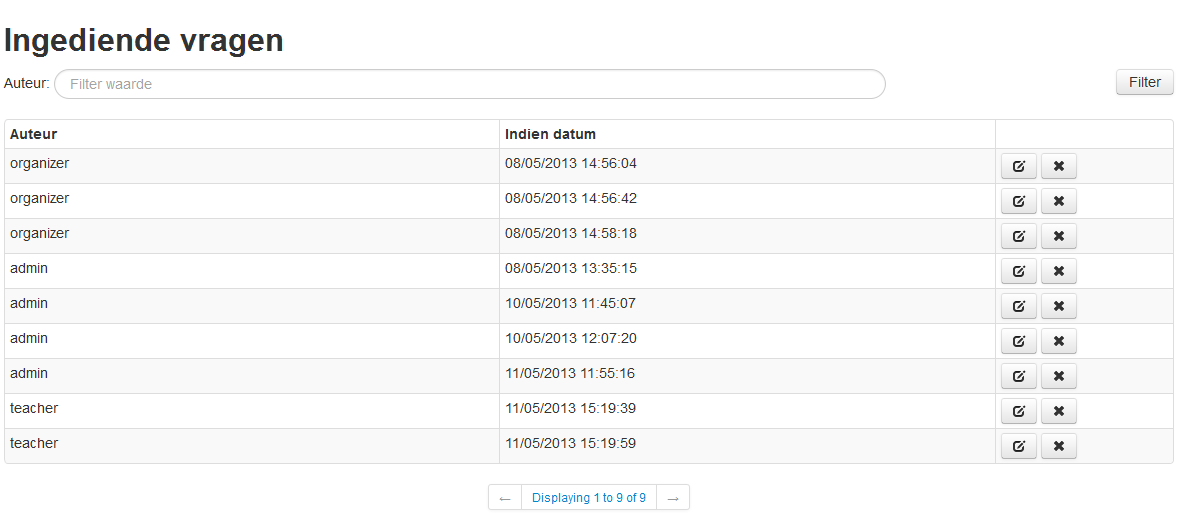
\includegraphics[width=1\textwidth]{img/questionsubmits}
	\caption{Ingediende vragen}
	\label{questionsubmits}
\end{figure}

Hier krijg je een overzicht van alle ingediende vragen met vermelding van de auteur en de indiendatum. Hier kan de organisator een vraag goedkeuren of afkeuren door op de desbetreffende knoppen te klikken. Bij het goedkeuren van een vraag, kent de organisator een officieel ID toe aan de vraag zodat deze later kan teruggevonden worden. Ook kiest hij een server waarop de vraag geplaatst wordt en bepaalt hij of de vraag momenteel actief is. Eens de vraag goedgekeurd is, wordt ze verwijderd uit de voorlopige lijst en toegevoegd aan de officiële lijst van vragen.

\textbf{\textit{Wat kan er mislopen?}}

Zorg er zeker voor dat de vraag een officieel ID krijgt toegekend.

\subsection{Wedstrijdbeheer}
Op deze pagina kan je de wedstrijden bekijken die voor jou zichtbaar zijn. 

\subsubsection{Nieuwe wedstrijd aanmaken}

\textbf{Stap 1}
Hier worden enkele gegevens gevraagd over de wedstrijd die je wenst aan te maken. 
Kies om te beginnen een naam voor de wedstrijd (vb. "`Bebras November 2011"'). Daarna kies je het type wedstrijd: Unrestricted, restricted of anoniem. Bepaal het start- en eindtijdstip van de wedstrijd met behulp van de datum- en tijdkiezer en vink het vakje aan om de wedstrijd te activeren.

\begin{figure}[!ht]
	\centering
	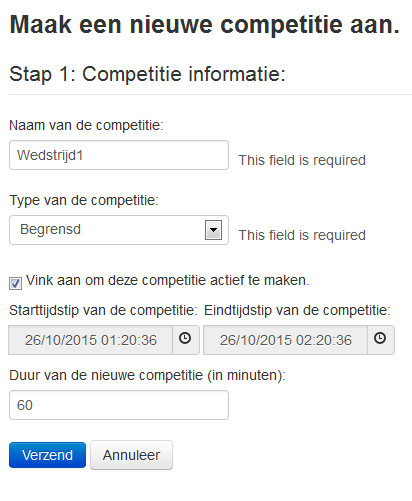
\includegraphics[width=0.5\textwidth]{img/stap1}
	\caption{Stap 1}
	\label{stap1}
\end{figure}

\textbf{Stap 2}
Hier worden enkele gegevens gevraagd over de vragenbundel die je wenst te gebruiken. 
Geef een naam voor de vragenbundel en bepaal het niveau. Je kan hiervoor kiezen uit de beschikbare leeftijdscategorie"en. Vink het vakje aan om deze vragenbundel actief te maken.

\begin{figure}[!ht]
	\centering
	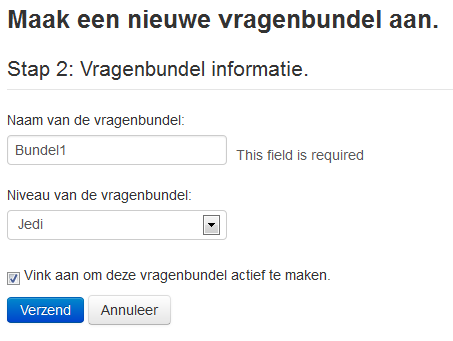
\includegraphics[width=0.5\textwidth]{img/stap2}
	\caption{Stap 2}
	\label{stap2}
\end{figure}

\textbf{Stap 3}
In stap 3 kun je de vragen selecteren die je wilt opnemen in de vragenbundel. Om een nieuwe vraag toe te voegen, klik je op 'Nieuw'. Hier kun je een vraag kiezen door het ID van de vraag in te geven. Selecteer een moeilijkheidsgraad uit de beschikbare opties en klik op 'Verzend'. De vraag zal nu in de vragenbundel opgenomen zijn. Wanneer je vragenbundel volledig is, klik je op 'Pas aan' om verder te gaan.

\begin{figure}[!ht]
	\centering
	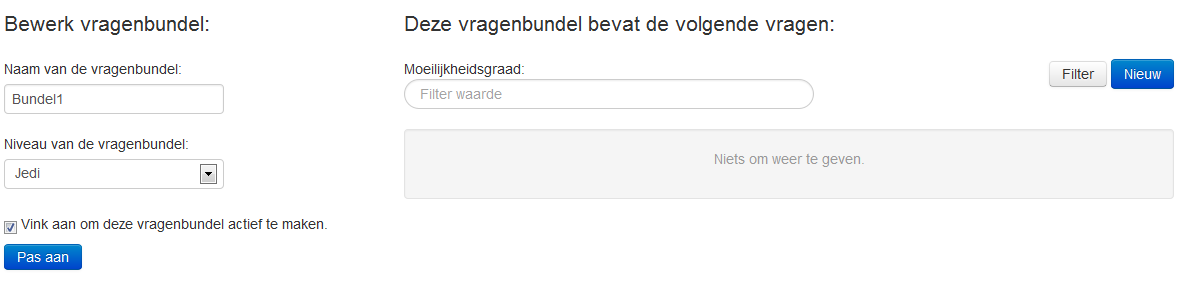
\includegraphics[width=1\textwidth]{img/stap3}
	\caption{Stap 3}
	\label{stap3}
\end{figure}

\textbf{\textit{Wat kan er mislopen?}}

Zorg er zeker voor dat de wedstrijd een naam, begin- en eindtijdstip krijgt toegekend. Ook de vragenbundel moet een naam krijgen.

\section{Administrator}

\subsection{Beheer Veelgestelde vragen}

\subsubsection{Bekijk veelgestelde vragen}
Deze pagina geeft een overzicht van alle veelgestelde vragen zoals te zien op figuur \ref{faq}.

\subsubsection{Bewerk veelgestelde vragen}

\begin{figure}[!ht]
	\centering
	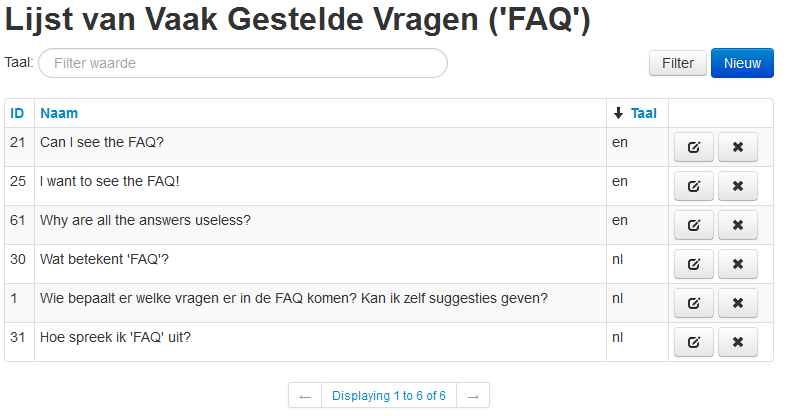
\includegraphics[width=1\textwidth]{img/faqmgmt}
	\caption{FAQ aanpassen}
	\label{faqmgmt}
\end{figure}

Op deze pagina zie je de lijst van alle veelgestelde vragen. Door op een kolomnaam te klikken, wordt de tabel automatisch op deze kolom gesorteerd. Om de volgorde om te draaien, klik je nogmaals op diezelfde kolomnaam. Door een taal in tegen, kan men de lijst filteren en enkel de vragen in die taal over houden. Onderaan de tabel kan men bladeren doorheen de lijst in het geval er meerdere pagina's met vragen zijn. Om een vraag te bewerken, klik je op de 'Bewerk'-knop. Een vraag verwijderen uit de lijst kan door op het kruisje te klikken.

\subsubsection{Maak een nieuwe veelgestelde vraag aan}

\begin{figure}[!ht]
	\centering
	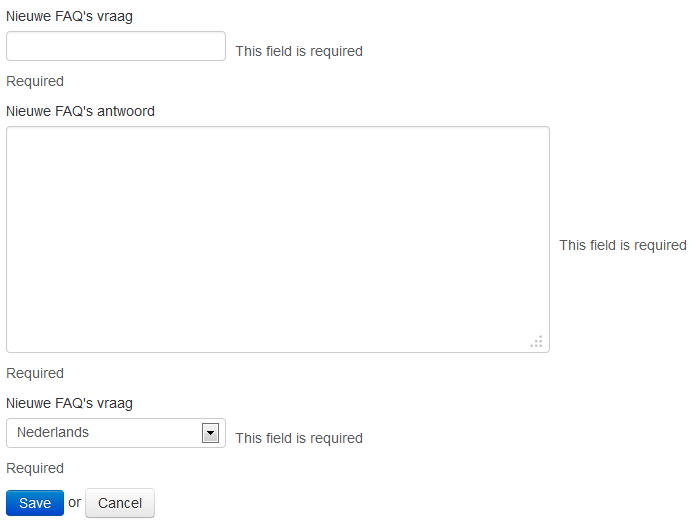
\includegraphics[width=1\textwidth]{img/new_faq}
	\caption{Nieuwe veelgestelde vraag}
	\label{new_faq}
\end{figure}

Om een nieuwe veelgestelde vraag toe te voegen, klik je op 'Voeg nieuwe FAQ toe'. [TODO: screenshot newFAQ] Op deze pagina vul je de vraag en het antwoord in in de daarvoor bestemde (en vereiste) velden. Daarna kies je de taal waarin de vraag is opgesteld en klik je op 'Save' om de vraag op te slaan. Je hebt ook de mogelijkheid om de vraag niet op te slaan en de actie te annuleren.

\textbf{\textit{Wat kan er mislopen?}}

Zorg er zeker voor dat alle verplichte velden zijn ingevuld.

\subsection{Pas de databank aan}

\subsubsection{Wijzig de navigatiebalk}

\begin{figure}[!ht]
	\centering
	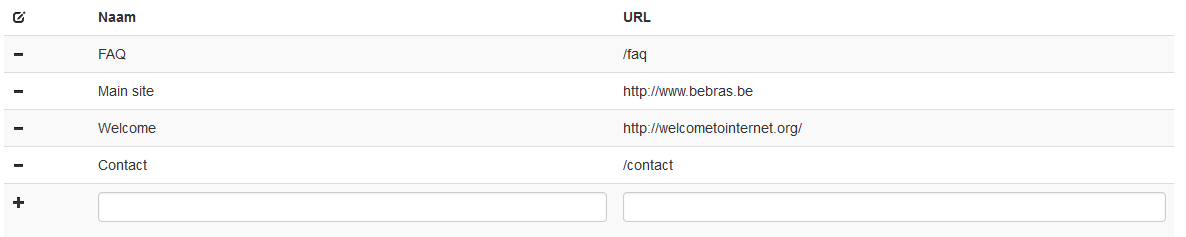
\includegraphics[width=1\textwidth]{img/homepage_links}
	\caption{Links wijzigen}
	\label{homepage_links}
\end{figure}

Hier kan de administrator de links wijzigen die de gebruikers linksbovenaan te zien krijgen. Om een nieuwe link toe te voegen, moet men de naam en de URL van de website in kwestie opgeven en vervolgens op de plus-knop klikken. Een site verwijderen uit de lijst kan door op de min-knop te klikken.

\subsubsection{Wijzig de leeftijdscategorieën}

\begin{figure}[!ht]
	\centering
	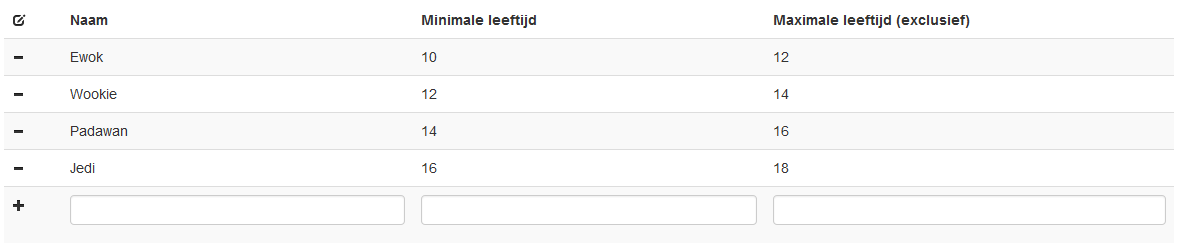
\includegraphics[width=1\textwidth]{img/age}
	\caption{Leeftijdscategorie"en wijzigen}
	\label{age}
\end{figure}

Hier kan de administrator de leeftijdscategorieën wijzigen. Om een nieuwe leeftijdscategorie toe te voegen, moet men de minimum- en maximumleeftijd opgeven en vervolgens op de plus-knop klikken. Een categorie verwijderen uit de lijst kan door op de min-knop te klikken.

\textbf{\textit{Wat kan er mislopen?}}

Alle verplichte velden moeten zeker ingevuld worden.

Zorg ervoor dat de minimumleeftijd jonger is dan de maximumleeftijd als je hierover een melding krijgt.

Als de naam voor de leeftijdscategorie al bestaat, kies dan een andere naam.

\subsubsection{Wijzig de moeilijkheidsgraden}

\begin{figure}[!ht]
	\centering
	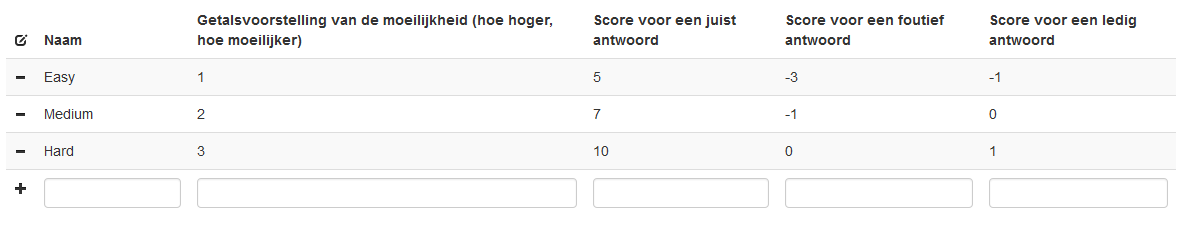
\includegraphics[width=1\textwidth]{img/difficulty}
	\caption{Moeilijkheidsgraden wijzigen}
	\label{difficulty}
\end{figure}

Hier kan de administrator de moeilijkheidsgraden wijzigen. Om een nieuwe moeilijkheidsgraad toe te voegen, moet men de naam en de rang meegeven die de moeilijkheid voorstelt en vervolgens op de plus-knop klikken. Een graad verwijderen uit de lijst kan door op de min-knop te klikken.

\textbf{\textit{Wat kan er mislopen?}}

Alle verplichte velden moeten zeker ingevuld worden.

Als de naam voor de moeilijkheidsgraad al bestaat, kies dan een andere naam.

\subsection{Boots gebruiker na}

\begin{figure}[!ht]
	\centering
	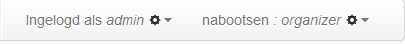
\includegraphics[width=0.5\textwidth]{img/mimic}
	\caption{Gebruiker nabootsen}
	\label{mimic}
\end{figure}

Om een gebruiker die lager in rang staat na te bootsen, heb je diens Bebras-ID nodig. Vul dit in in het daarvoor bestemde veld en klik dan op 'Mimic'. Nu heb je toegang tot de account van de gebruiker die je wilt imiteren. Dit is zichtbaar rechtsboven waar je naast je eigen ingelogde status nu ook de ge"imiteerde gebruiker ziet staan. De admin kan elke gebruiker nabootsen, de organizer iedereen behalve de admin en leerkrachten kunnen enkel hun eigen actieve leerlingen imiteren. Indien je een account probeert na te bootsen waar je geen toegangsrechten tot hebt, zal je hiervan een melding krijgen. Het is mogelijk om via een ge"imiteerde account een andere account te imiteren. Om terug te keren naar je originele account, meld je je af bij de nagebootste account. Zo kom je terug op jouw startpagina. 

\end{document}